\part{Outils pour les probabilités}

\section{Factorielle}\label{factoriel}

\subsection{Idée}

\begin{tipblock}
\cmaj{3.04a} L'idée est de proposer de quoi travailler avec les factorielles.

Les calculs sont effectués par le package \ctex{xint}, et le formatage peut être effectué par le package \ctex{siunitx}.
\end{tipblock}

\begin{PresCodeTexPL}{listing only}
\Factorielle(*)[clés]{nb}
\end{PresCodeTexPL}

\begin{PresCodePL}{}
\Factorielle{9}\\
\Factorielle{17}
\end{PresCodePL}

\subsection{Clés}

\begin{cautionblock}
La version \textit{étoilée} ne formate pas les résultats par \ctex{siunitx}.

\smallskip

Les \Cle{clés} disponibles pour cette commande sont :

\begin{itemize}
	\item \DescripCle[false]{Enonce}{booléen pour afficher l'énoncé}
	\item \DescripCle[false]{Partiel}{booléen pour afficher la formule partielle}
	\item \DescripCle[false]{Complet}{booléen pour afficher la formule complète}
	\item \DescripCle[false]{Grand}{booléen pour les grands résultats}
	\item \DescripCle[m]{Sens}{préciser l'ordre pour les détails \Cle{d/m}}
	\item \DescripCle*[9]{ChSignif}{nombre de chiffres significatifs pour les grands résultats}
	\item \DescripCle[\textbackslash mkern1.5mu\textbackslash relax1.5]{Espace}{espace avant le \og ! \fg}
\end{itemize}
\vspace*{-\baselineskip}\leavevmode
\end{cautionblock}

\begin{PresCodePL}{}
\Factorielle[Enonce,Complet]{9}
\end{PresCodePL}

\begin{PresCodePL}{}
\Factorielle[Enonce,Complet,Sens=d]{9}
\end{PresCodePL}

\begin{PresCodePL}{}
\Factorielle[Enonce,Partiel]{9}
\end{PresCodePL}

\begin{PresCodePL}{}
\Factorielle[Enonce,Partiel,Sens=d]{9}
\end{PresCodePL}

\begin{PresCodePL}{}
\Factorielle[Grand,Enonce,Partiel]{147}
\end{PresCodePL}

\newpage

\section{Calculs de probabilités}\label{calcprobas}

\subsection{Introduction}

\begin{tipblock}
L'idée est de proposer des commandes permettant de calculer des probabilités avec des lois classiques :

\begin{itemize}
	\item binomiale ;
	\item normale ;
	\item exponentielle ;
	\item de Poisson ;
	\item géométrique ;
	\item hypergéométrique.
\end{itemize}
\vspace*{-\baselineskip}\leavevmode
\end{tipblock}

\begin{noteblock}
Les commandes sont de deux natures :

\begin{itemize}
	\item des commandes pour calculer, grâce au package \ctex{xintexpr} ;
	\item des commandes pour formater le résultat de \ctex{xintexpr}, grâce à \ctex{siunitx}.
\end{itemize}

De ce fait, les options de \ctex{siunitx} de l'utilisateur affecterons les formatages du résultat, la commande va \og forcer \fg{} les arrondis et l'écriture scientifique.
\end{noteblock}

\subsection{Calculs \og simples \fg}

\begin{PresCodeTexPL}{listing only}
%loi binomiale B(n,p)
\CalcBinomP{n}{p}{k}             %P(X=k)
\CalcBinomC{n}{p}{a}{b}          %P(a<=X<=b)

%loi de Poisson P(l)
\CalcPoissP{l}{k}                %P(X=k)
\CalcPoissC{l}{a}{b}             %P(a<=X<=b)

%loi géométrique G(p)
\CalcGeomP{p}{k}                 %P(X=k)
\CalcGeomC{l}{a}{b}              %P(a<=X<=b)

%loi hypergéométrique H(N,n,m)
\CalcHypergeomP{N}{n}{m}{k}      %P(X=k)
\CalcHypergeomP{N}{n}{m}{a}{b}   %P(a<=X<=b)

%loi normale N(m,s)
\CalcNormC{m}{s}{a}{b}           %P(a<=X<=b)

%loi exponentielle E(l)
\CalcExpoC{l}{a}{b}              %P(a<=X<=b)
\end{PresCodeTexPL}

\begin{cautionblock}
Les probabilités calculables sont donc -- comme pour beaucoup de modèles de calculatrices -- les probabilités \textbf{P}onctuelles ($P(X=k)$) et \textbf{C}umulées ($P(a\leqslant X\leqslant b)$).

\smallskip

Pour les probabilités cumulées, on peut utiliser le caractère \ctex{*} comme borne ($a$ ou $b$), pour les probabilités du type $P(X\leqslant b)$ et $P(X \geqslant a)$.
\end{cautionblock}

\begin{PresCodeTexPL}{listing only}
% X -> B(5,0.4)
$P(X=3) \approx \CalcBinomP{5}{0.4}{3}$.
$P(X\leqslant1) \approx \CalcBinomC{5}{0.4}{*}{1}$.

% X -> B(100,0.02)
$P(X=10) \approx \CalcBinomP{100}{0.02}{10}$.
$P(15\leqslant X\leqslant25) \approx \CalcBinomC{100}{0.02}{15}{25}$.

% Y -> P(5)
$P(Y=3) \approx \CalcPoissP{5}{3}$.
$P(Y\geqslant2) \approx \CalcPoissC{5}{2}{*}$.

% T -> G(0.5)
$P(T=100) \approx \CalcPoissP{0.5}{3}$.
$P(T\leqslant5) \approx \CalcPoissC{0.5}{*}{5}$.

% W -> H(50,10,5)
$P(W=4) \approx \CalcHypergeomP{50}{10}{5}{4}$.
$P(1\leqslant W\leqslant3) \approx \CalcHypergeomC{50}{10}{5}{1}{3}$.
\end{PresCodeTexPL}

\begin{PresCodeSortiePL}{text only}
$\bullet~~~~X \hookrightarrow \mathcal{B}(5\,; 0,4)$ :\\
$P(X=3) \approx \CalcBinomP{5}{0.4}{3}$.\\
$P(X\leqslant1) \approx \CalcBinomC{5}{0.4}{*}{1}$.

\medskip

$\bullet~~~~X \hookrightarrow \mathcal{B}(100\,; 0,02)$ :\\
$P(X=10) \approx \CalcBinomP{100}{0.02}{10}$.\\
$P(15\leqslant X\leqslant25) \approx \CalcBinomC{100}{0.02}{15}{25}$.

\medskip

$\bullet~~~~Y \hookrightarrow \mathcal{P}_5$ :\\
$P(Y=3) \approx \CalcPoissP{5}{3}$.\\
$P(Y\geqslant2) \approx \CalcPoissC{5}{2}{*}$.

\medskip

$\bullet~~~~T \hookrightarrow \mathcal{G}_{0,5}$ :\\
$P(T=3) \approx \CalcGeomP{0.5}{3}$.\\
$P(T\leqslant5) \approx \CalcGeomC{0.5}{*}{5}$.

\medskip

$\bullet~~~~W \hookrightarrow \mathcal{H}(50\,; 10\,; 5)$ :\\
$P(W=4) \approx \CalcHypergeomP{50}{10}{5}{4}$.\\
$P(1\leqslant W\leqslant3) \approx \CalcHypergeomC{50}{10}{5}{1}{3}$.
\end{PresCodeSortiePL}

\begin{PresCodeTexPL}{listing only}
% X -> N(0,1)
$P(X\leqslant1) \approx \CalcNormC{0}{1}{*}{1}$.
$P(-1,96\leqslant Z\leqslant1,96) \approx \CalcNormC{0}{1}{-1.96}{1.96}$.

% X -> N(550,30)
$P(Y\geqslant600) \approx \CalcNormC{550}{30}{600}{*}$.
$P(500\leqslant Y\leqslant600) \approx \CalcNormC{550}{30}{500}{600}$.

% Z -> E(0.001)
$P(Z\geqslant400) \approx \CalcExpoC{0.001}{400}{*}$.
$P(300\leqslant Z\leqslant750) \approx \CalcExpoC{0.001}{300}{750}$.
\end{PresCodeTexPL}

\begin{PresCodeSortiePL}{text only}
$\bullet~~~~X \hookrightarrow \mathcal{N}(0\,; 1)$ :\\
$P(X\leqslant1) \approx \CalcNormC{0}{1}{*}{1}$.\\
$P(-1,96\leqslant Z\leqslant1,96) \approx \CalcNormC{0}{1}{-1.96}{1.96}$.

\medskip

$\bullet~~~~Y \hookrightarrow \mathcal{N}(550\,; 30)$ :\\
$P(Y\geqslant600) \approx \CalcNormC{550}{30}{600}{*}$.\\
$P(500\leqslant Y\leqslant600) \approx \CalcNormC{550}{30}{500}{600}$.

\medskip

$\bullet~~~~Z \hookrightarrow \mathcal{E}_{0,001}$ :\\
$P(Z\geqslant400) \approx \CalcExpoC{0.001}{400}{*}$.\\
$P(300\leqslant Z\leqslant750) \approx \CalcExpoC{0.001}{300}{750}$.
\end{PresCodeSortiePL}

\subsection{Complément avec sortie \og formatée \fg}

\begin{tipblock}
L'idée est ensuite de formater le résultat obtenu par \ctex{xintexpr}, pour un affichage homogène.

\smallskip

L'utilisateur peut donc utiliser \og sa \fg{} méthode pour formater les résultats obtenus par \ctex{xintexpr} !
\end{tipblock}

\begin{PresCodeTexPL}{listing only}
%avec un formatage manuel
\num[exponent-mode=scientific]{\CalcBinomP{100}{0.02}{10}}
\end{PresCodeTexPL}

\begin{PresCodePL}{}
$\bullet~~~~X \hookrightarrow \mathcal{B}(100\,; 0,02)$ :

$P(X=10) \approx \num[exponent-mode=scientific]{\CalcBinomP{100}{0.02}{10}}$.
\end{PresCodePL}

\begin{tipblock}
Le package \ctex{ProfLycee} propose -- en complément -- des commandes pour formater, grâce à \ctex{siunitx}, le résultat.

Les commandes ne sont donc, dans ce cas, pas préfixées par \ctex{calc} :

\begin{itemize}
	\item formatage sous forme décimale \textit{pure} : $0,00\ldots$ ;
	\item formatage sous forme scientifique : $n,\ldots\times10^{\ldots}$.
\end{itemize}
\vspace*{-\baselineskip}\leavevmode
\end{tipblock}

\begin{PresCodeTexPL}{listing only}
%loi binomiale B(n,p)
\BinomP(*)[prec]{n}{p}{k}         %P(X=k)
\BinomC(*)[prec]{n}{p}{a}{b}      %P(a<=X<=b)

%loi de Poisson P (l)
\PoissonP(*)[prec]{l}{k}          %P(X=k)
\PoissonC(*)[prec]{l}{a}{b}       %P(a<=X<=b)

%loi géométrique G (p)
\GeomP{p}{k}                      %P(X=k)
\GeomC{l}{a}{b}                   %P(a<=X<=b)

%loi hypergéométrique H (N,n,m)
\HypergeomP{N}{n}{m}{k}           %P(X=k)
\HypergeomC{N}{n}{m}{a}{b}        %P(a<=X<=b)

%loi normale N(m,s)
\NormaleC(*)[prec]{m}{s}{a}{b}    %P(a<=X<=b)

%loi exponentielle E(l)
\ExpoC(*)[prec]{l}{a}{b}          %P(a<=X<=b)
\end{PresCodeTexPL}

\begin{cautionblock}
Quelques précisions sur les commandes précédentes :

\begin{itemize}
	\item la version étoilée \Cle{*} des commandes formate le résultat en mode scientifique ;
	\item l'argument optionnel (par défaut \Cle{3}) correspond à quant à lui à l'arrondi.
\end{itemize}
\vspace*{-\baselineskip}\leavevmode
\end{cautionblock}

\begin{PresCodeTexPL}{listing only}
% X -> N(550,30)
$P(Y\geqslant600) \approx \NormaleC[4]{550}{30}{600}{*}$.
$P(500\leqslant Y\leqslant600) \approx \NormaleC[4]{550}{30}{500}{600}$.
% X -> B(100,0.02)
$P(X=10) \approx \BinomP[7]{100}{0.02}{10} \approx \BinomP*[7]{100}{0.02}{10}$.
$P(15\leqslant X\leqslant25) \approx \BinomC[10]{100}{0.02}{15}{25} \approx \BinomC*[10]{100}{0.02}{15}{25}$.
% H -> H(50,10,5)
$P(W=4) \approx \HypergeomP[5]{50}{10}{5}{4}$.
$P(1\leqslant W\leqslant3) \approx \HypergeomC[4]{50}{10}{5}{1}{3}$.
% Z-> E(0,001)$ :
$P(Z\geqslant400) \approx \ExpoC{0.001}{400}{*}$.
$P(300\leqslant Z\leqslant750) \approx \ExpoC{0.001}{300}{750}$.
% T -> P(5)
$P(T=3) \approx \PoissonP{5}{3}$.
$P(T\geqslant2) \approx \PoissonC[4]{5}{2}{*}$.
\end{PresCodeTexPL}

\begin{PresCodeSortiePL}{text only}
$\bullet~~~~Y \hookrightarrow \mathcal{N}(550\,; 30)$ :

$P(Y\geqslant600) \approx \NormaleC[4]{550}{30}{600}{*}$.

$P(500\leqslant Y\leqslant600) \approx \NormaleC[4]{550}{30}{500}{600}$.

\medskip

$\bullet~~~~X \hookrightarrow \mathcal{B}(100\,; 0,02)$ :

$P(X=10) \approx \BinomP[7]{100}{0.02}{10} \approx \BinomP*[7]{100}{0.02}{10}$.

$P(15\leqslant X\leqslant25) \approx \BinomC[10]{100}{0.02}{15}{25} \approx \BinomC*[10]{100}{0.02}{15}{25}$.

\medskip

$\bullet~~~~W \hookrightarrow \mathcal{H}(50\,; 10\,; 5)$ :

$P(W=4) \approx \HypergeomP[5]{50}{10}{5}{4}$.

$P(1\leqslant W\leqslant3) \approx \HypergeomC[4]{50}{10}{5}{1}{3}$.

\medskip

$\bullet~~~~Z \hookrightarrow \mathcal{E}_{0,001}$ :

$P(Z\geqslant400) \approx \ExpoC{0.001}{400}{*}$.

$P(300\leqslant Z\leqslant750) \approx \ExpoC{0.001}{300}{750}$.

\medskip

$\bullet~~~~T \hookrightarrow \mathcal{P}_5$ :

$P(T=3) \approx \PoissonP{5}{3}$.

$P(T\geqslant2) \approx \PoissonC[4]{5}{2}{*}$.
\end{PresCodeSortiePL}

\begin{noteblock}
\hfill~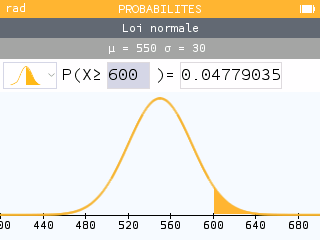
\includegraphics[height=3cm]{./graphics/pl-doc-probas_a}~~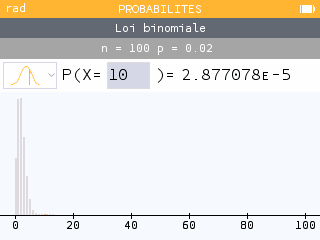
\includegraphics[height=3cm]{./graphics/pl-doc-probas_c}~~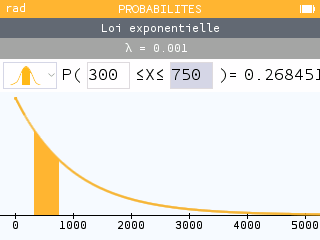
\includegraphics[height=3cm]{./graphics/pl-doc-probas_e}~~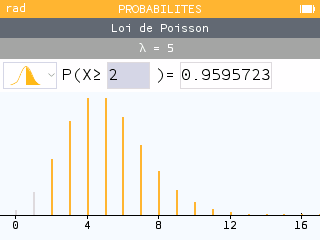
\includegraphics[height=3cm]{./graphics/pl-doc-probas_f}\hfill~
\end{noteblock}

\newpage

\section{Arbres de probabilités \og classiques \fg}\label{arbresprobas}

\subsection{Introduction}

\begin{tipblock}
L'idée est de proposer des commandes pour créer des arbres de probabilités classiques (et homogènes), en \TikZ, de format :

\begin{itemize}
	\item $2\times2$ ou $2\times3$ ;
	\item $3\times2$ ou $3\times3$.
\end{itemize}

Les (deux) commandes sont donc liées à un environnement \ctex{tikzpicture}, et elles créent les nœuds de l'arbre, pour exploitation ultérieure éventuelle.
\end{tipblock}

\begin{PresCodeTexPL}{listing only}
%commande simple pour tracé de l'arbre
\ArbreProbasTikz[options]{donnees}

%environnement pour tracé et exploitation éventuelle
\begin{EnvArbreProbasTikz}[options]{donnees}
	code tikz supplémentaire
\end{EnvArbreProbasTikz}
\end{PresCodeTexPL}

\subsection{Options et arguments}

\begin{noteblock}
Les \Cle{donnees} seront à préciser sous forme

\hfill\ctex{<sommet1>/<proba1>/<position1>,<sommet2>/<proba2>/<position2>,...}\hfill~

avec comme \og sens de lecture \fg{} de la gauche vers la droite puis du haut vers le bas (on balaye les \textit{sous-arbres}), avec comme possibilités :

\begin{itemize}
	\item \cmaj{2.5.3} une donnée \Cle{proba} peut être laissée vide ou spécifiée avec des \textsf{macros} ;
	\item une donnée \Cle{position} peut valoir \Cle{above} (au-dessus), \Cle{below} (en-dessous) ou être laissée \Cle{vide} (sur) ;
	\item \cmaj{3.02b} la clé \Cle{PositionProbas} (vide par défaut) peut permettre de positionner toutes les probas suivant :
	\begin{itemize}
		\item \Cle{auto} := position automatique des probas ;
		\item \Cle{dessus} := position au-dessus des branches ;
		\item \Cle{dessous} := position au-dessous des branches ;
		\item \Cle{sur} := position sur les branches.
	\end{itemize}
\end{itemize}
\vspace*{-\baselineskip}\leavevmode
\end{noteblock}

\begin{cautionblock}
Quelques \Cle{Clés} (communes) pour les deux commandes :

\begin{itemize}
	\item la clé \Cle{Unite} pour préciser l'unité de l'environnement \TikZ{} ; \hfill~défaut \Cle{1cm}
	\item la clé \Cle{EspaceNiveau} pour l'espace (H) entre les étages ; \hfill~défaut \Cle{3.25}
	\item la clé \Cle{EspaceFeuille} pour l'espace (V) entre les feuilles ; \hfill~défaut \Cle{1}
	\item la clé \Cle{Type} pour le format, parmi \Cle{2x2} ou \Cle{2x3} ou \Cle{3x2} ou  \Cle{3x3} ; \hfill~défaut \Cle{2x2}
	\item la clé \Cle{Police} pour la police des nœuds ; \hfill~défaut \Cle{\textbackslash{}normalfont\textbackslash{}normalsize}
	\item la clé \Cle{PoliceProbas} pour la police des probas ; \hfill~défaut \Cle{\textbackslash{}normalfont\textbackslash{}small}
	\item le booléen \Cle{InclineProbas} pour incliner les probas ; \hfill~défaut \Cle{true}
	\item la clé \Cle{Racine} pour afficher une racine ; \hfill~défaut \Cle{vide}
	\item le booléen \Cle{Fleche} pour afficher une flèche sur les branches ; \hfill~défaut \Cle{false}
	\item la clé \Cle{StyleTrait} pour les branches, en langage \TikZ{} ; \hfill~défaut \Cle{vide}
	\item la clé \Cle{EpaisseurTrait} pour l'épaisseur des branches, en langage \TikZ{} ; \hfill~défaut \Cle{semithick}
\end{itemize}
\vspace*{-\baselineskip}\leavevmode
\end{cautionblock}

\begin{PresCodeTexPL}{listing only}
\def\ArbreDeuxDeux{
		$A$/\num{0.5}/,
			$B$/\num{0.4}/,
			$\overline{B}$/.../,
		$\overline{A}$/.../,
			$B$/.../,
			$\overline{B}$/$\frac{1}{3}$/
	}

\ArbreProbasTikz{\ArbreDeuxDeux}

%des éléménts, en gris, ont été rajoutés pour illustrer certaines options
\end{PresCodeTexPL}

\begin{PresCodeSortiePL}{text only}
\begin{EnvArbreProbasTikz}{$A$/\num{0.5}/,$B$/\num{0.4}/,$\overline{B}$/.../,$\overline{A}$/.../,$B$/.../,$\overline{B}$/$\frac{1}{3}$/}
	\draw[lightgray] (R) node[left,font=\ttfamily\small] {(R)} ;
	\draw[lightgray] (A11) node[below,font=\ttfamily\small] {(A11)} ;
	\draw[lightgray] (A12) node[below,font=\ttfamily\small] {(A12)} ;
	\draw[lightgray] (A21) node[below,font=\ttfamily\small] {(A21)} ;
	\draw[lightgray] (A22) node[below,font=\ttfamily\small] {(A22)} ;
	\draw[lightgray] (A23) node[below,font=\ttfamily\small] {(A23)} ;
	\draw[lightgray] (A24) node[below,font=\ttfamily\small] {(A24)} ;
	\draw[lightgray,<->,>=latex] (0,-4) -- (3.25,-4) node[midway,below,font=\ttfamily\small] {EspaceNiveau} ;
	\draw[lightgray,<->,>=latex] (3.25,-4) -- (6.5,-4) node[midway,below,font=\ttfamily\small] {EspaceNiveau} ;
	\draw[lightgray,<->,>=latex] (7,0) -- (7,-1) node[midway,right,font=\ttfamily\small] {EspaceFeuille} ;
	\draw[lightgray,<->,>=latex] (7,-1) -- (7,-2) node[midway,right,font=\ttfamily\small] {EspaceFeuille} ;
	\draw[lightgray,<->,>=latex] (7,-2) -- (7,-3) node[midway,right,font=\ttfamily\small] {EspaceFeuille} ;
\end{EnvArbreProbasTikz}
\end{PresCodeSortiePL}

\begin{noteblock}
Les nœuds crées par les commandes sont :

\begin{itemize}
	\item \ctex{R} pour la racine ;
	\item \ctex{A1x} pour les nœuds du 1\up{er} niveau (de haut en bas) ;
	\item  \ctex{A2x} pour les nœuds du 2\up{d} niveau (de haut en bas).
\end{itemize}
\vspace*{-\baselineskip}\leavevmode
\end{noteblock}

\subsection{Exemples complémentaires}

\begin{tipblock}
\cmaj{3.04g} À noter qu'il existe les clés \Cle{CouleurTraits},\Cle{CouleurNoeuds} et \Cle{CouleurProbas} pour personnaliser un peu plus en profondeur l'arbre de probabilités. 
\end{tipblock}

\begin{PresCodeTexPL}{listing only}
\def\ArbreTroisDeux{
	$A_1$/\num{0.5}/,
		$B$/\num{0.4}/,
		$\overline{B}$/\numdots/,
	$A_2$/\numdots/,
		$B$/\numdots/,
		$\overline{B}$/$\frac{1}{3}$/,
	$A_3$/\numdots/,
		$B$/\numdots./,
		$\overline{B}$/$\frac{4}{15}$/
}

\begin{EnvArbreProbasTikz}
	[Type=3x2,Fleche,EspaceNiveau=5,EspaceFeuille=1.25,PositionProbas=auto]%
	{\ArbreTroisDeux}
	\draw[CouleurVertForet,->] (A24)--($(A24)+(2.5,0)$) node[right,font=\sffamily] {code tikz rajouté} ;
\end{EnvArbreProbasTikz}
\end{PresCodeTexPL}

\begin{PresCodeSortiePL}{text only}
\begin{EnvArbreProbasTikz}[Type=3x2,Fleche,EspaceNiveau=5,EspaceFeuille=1.25,PositionProbas=auto]{$A_1$/\num{0.5}/,$B$/\num{0.4}/,$\overline{B}$/\numdots/,$A_2$/\numdots/,$B$/\numdots/,$\overline{B}$/$\frac{1}{3}$/,$A_3$/\numdots/,$B$/\numdots/,$\overline{B}$/$\frac{4}{15}$/}
	\draw[CouleurVertForet,->] (A24)--($(A24)+(2.5,0)$) node[right,font=\sffamily] {code tikz rajouté} ;
\end{EnvArbreProbasTikz}
\end{PresCodeSortiePL}

\begin{PresCodeTexPL}{listing only}
\def\ArbreDeuxTrois{
	$A$/\num{0.05}/above,
		$B_1$/\num{0.4}/above,$B_2$/\num{0.35}/,$B_3$//below,
	$\overline{A}$/.../below,
		$B_1$/$\frac{2}{15}$/above,$B_2$/.../,$B_3$/$\frac{1}{3}$/below
}
\ArbreProbasTikz[Type=2x3,InclineProbas=false,EspaceFeuille=1.15]{\ArbreDeuxTrois}

\def\ArbreTroisTrois{
		$A_1$/\num{0.05}/,$B_1$/{1/3}/,$B_2$/{1/3}/,$B_3$/{1/3}/,
		$A_2$/\num{0.80}/,$B_1$/{1/3}/,$B_2$/{1/3}/,$B_3$/{1/3}/,
		$A_3$/\num{0.15}/,$B_1$/{1/3}/,$B_2$/{1/3}/,$B_3$/{1/3}/
	}

\ArbreProbasTikz%
	[Type=3x3,StyleTrait={densely dashed},
	CouleurTraits=red,CouleurProbas=blue,CouleurNoeuds=olive,
	EspaceFeuille=0.7,PoliceProbas=\scriptsize,Police=\small]%
	{\ArbreTroisTrois}
\end{PresCodeTexPL}

\begin{PresCodeSortiePL}{text only}
\ArbreProbasTikz[Type=2x3,InclineProbas=false,EspaceFeuille=1.15]{$A$/\num{0.05}/above,$B_1$/\num{0.4}/above,$B_2$/\num{0.35}/,$B_3$//below,$\overline{A}$/.../below,$B_1$/$\frac{2}{15}$/above,$B_2$/.../,$B_3$/$\frac{1}{3}$/below}
~~
\ArbreProbasTikz[Type=3x3,StyleTrait={densely dashed},EspaceFeuille=0.7,PoliceProbas=\scriptsize,Police=\small,CouleurTraits=red,CouleurProbas=blue,CouleurNoeuds=olive]{$A_1$/\num{0.05}/,$B_1$/{1/3}/,$B_2$/{1/3}/,$B_3$/{1/3}/,$A_2$/\num{0.80}/,$B_1$/{1/3}/,$B_2$/{1/3}/,$B_3$/{1/3}/,$A_3$/\num{0.15}/,$B_1$/{1/3}/,$B_2$/{1/3}/,$B_3$/{1/3}/}
\end{PresCodeSortiePL}

\newpage

\section{Petits schémas pour des probabilités continues}\label{schemasprobas}

\subsection{Idée}

\begin{tipblock}
L'idée est de proposer des commandes pour illustrer, sous forme de schémas en \TikZ, des probabilités avec des lois continues (normales et exponentielles).

\smallskip

Ces \og schémas \fg{} peuvent être insérés en tant que graphique explicatif, ou bien en tant que petite illustration rapide !
\end{tipblock}

\begin{PresCodeTexPL}{listing only}
\LoiNormaleGraphe[options]<options tikz>{m}{s}{a}{b}

\LoiExpoGraphe[options]<options tikz>{l}{a}{b}
\end{PresCodeTexPL}

\begin{PresCodeSortiePL}{text only}
\hfill\LoiNormaleGraphe{100}{20}{80}{120}\hspace{3cm}\LoiExpoGraphe{0.001}{250}{1500}\hfill~
\end{PresCodeSortiePL}

\begin{cautionblock}
Les probabilités \textit{illustrables} sont donc des probabilités \textbf{C}umulées ($P(a\leqslant X\leqslant b)$).

\smallskip

On peut utiliser \ctex{*} comme borne ($a$ ou $b$), pour les probabilités du type $P(X\leqslant b)$ et $P(X \geqslant a)$.
\end{cautionblock}

\subsection{Commandes et options}

\begin{cautionblock}
Quelques \Cle{Clés} sont disponibles pour ces commandes :

\begin{itemize}
	\item la clé \Cle{CouleurAire} pour l'aire sous la courbe ; \hfill{}défaut \Cle{LightGray}
	\item la clé \Cle{CouleurCourbe} pour la courbe ; \hfill{}défaut \Cle{red}
	\item la clé \Cle{Largeur} qui sera la largeur (en cm) du graphique ; \hfill{}défaut \Cle{2}
	\item la clé \Cle{Hauteur} qui sera la hauteur (en cm) du graphique ; \hfill{}défaut \Cle{1}
	\item un booléen \Cle{AfficheM} qui affiche la moyenne ; \hfill{}défaut \Cle{true}
	\item un booléen \Cle{AfficheCadre} qui affiche un cadre pour délimiter le schéma. \hfill{}défaut \Cle{true}
\end{itemize}
\vspace*{-\baselineskip}\leavevmode
\end{cautionblock}

\begin{noteblock}
Les commandes sont donc des environnements \TikZ, sans possibilité de \og rajouter \fg{} des éléments. Ces petis \textit{schémas} sont donc vraiment dédiés à \textit{montrer} rapidement une probabilité continue, sans fioriture.
\end{noteblock}

\begin{PresCodePL}{}
Avec centrage vertical sur l'axe des abscisses :
\LoiNormaleGraphe
	[AfficheM=false,CouleurCourbe=blue,CouleurAire=cyan]<baseline=0pt>%
	{1000}{100}{950}{*}
\end{PresCodePL}

\begin{PresCodePL}{}
Avec quelques modifications :

\LoiNormaleGraphe[Largeur=4,Hauteur=2]{150}{12.5}{122}{160}

\medskip

Avec centrage vertical :
\LoiNormaleGraphe[Largeur=5,Hauteur=2.5]<baseline=(current bounding box.center)>{200}{5}{204}{*}

\medskip

Avec centrage vertical sur l'axe des abscisses :
\LoiExpoGraphe
	[AfficheM=false,CouleurCourbe=blue,CouleurAire=cyan]<baseline=0pt>{0.05}{*}{32}

\medskip

\LoiExpoGraphe[Largeur=4,Hauteur=2]{0.00025}{5000}{*}
\end{PresCodePL}

\subsection{Remarques et compléments}

\begin{noteblock}
Pour le moment, seules les lois (continues) exponentielles et normales sont disponibles, peut-être que d'autres lois seront ajoutées, mais il ne me semble pas très pertinent de proposer des schémas similaires pour des lois discrètes, qui ont des \textit{représentations} assez variables\ldots
\end{noteblock}

\newpage

\section{Nombres aléatoires}\label{entiersaleatoires}

\subsection{Idée}

\begin{tipblock}
\cmaj{2.0.9} L'idée est de proposer des commandes pour générer des nombres aléatoires, pour exploitation ultérieure :

\begin{itemize}
	\item un entier ou un nombre décimal ;
	\item des nombres entiers, avec ou sans répétitions.
\end{itemize}
\vspace*{-\baselineskip}\leavevmode
\end{tipblock}

\begin{noteblock}
Pour chacune des commandes, le ou les résultats sont stockés dans une \textsf{macro} dont le nom est choisi par l'utilisateur.
\end{noteblock}

\begin{PresCodeTexPL}{listing only}
%entier aléatoire entre a et b
\NbAlea{a}{b}{macro}

%nombre décimal (n chiffres après la virgule) aléatoire entre a et b+1 (exclus)
\NbAlea[n]{a}{b}{macro}

%création d'un nombre aléatoire sous forme d'une macro
\VarNbAlea{macro}{calculs}

%liste d'entiers aléatoires
\TirageAleatoireEntiers[options]{macro}
\end{PresCodeTexPL}

\begin{PresCodePL}{}
%nombre aléatoire entre 1 et 50, stocké dans \PremierNbAlea
Entier entre 1 et 50 : \NbAlea{1}{50}{\PremierNbAlea}\PremierNbAlea \\
%nombre aléatoire créé à partir du 1er, stocké dans \DeuxiemeNbAlea
Entier à partir du précédent : \VarNbAlea{\DeuxiemeNbAlea}{\PremierNbAlea+randint(0,10)}\DeuxiemeNbAlea \\
%nombre aléatoire décimal (au millième) entre 0 et 10+1 (exclus), stocké dans \PremierDecAlea
Décimal entre 0 et $10,999\ldots$ : \NbAlea[3]{0}{10}{\PremierDecAlea}\PremierDecAlea \\
%liste de 6 nombres, sans répétitions, entre 1 et 50
Liste par défaut (6 entre 1 et 50) : \TirageAleatoireEntiers{\PremiereListeAlea}\PremiereListeAlea
\end{PresCodePL}

\begin{noteblock}
Les listes créées sont exploitables, \textit{a posteriori}, par le package \ctex{listofitems} par exemple !
\end{noteblock}

\begin{PresCodePL}{}
Liste générée : \TirageAleatoireEntiers{\TestListeA}\TestListeA

Liste traitée : \readlist*\LISTEa{\TestListeA}\showitems{\LISTEa}
\end{PresCodePL}

\pagebreak

\subsection{Clés et options}

\begin{cautionblock}
Quelques clés sont disponibles pour la commande \ctex{TirageAleatoireEntiers} :

\begin{itemize}
	\item la clé \Cle{ValMin} pour préciser borne inférieure de l'intervalle ;\hfill{}défaut \Cle{1}
	\item la clé \Cle{ValMax} pour préciser borne supérieure de l'intervalle ;\hfill{}défaut \Cle{50}
	\item la clé \Cle{NbVal} qui est le nombre d'entiers à générer ;\hfill{}défaut \Cle{6}
	\item la clé \Cle{Sep} pour spécifier le séparateur d'éléments ;\hfill{}défaut \Cle{,}
	\item la clé \Cle{Tri} parmi \Cle{non/croissant/decroissant} pour trier les valeurs
	;\hfill{}défaut \Cle{non}
	\item le booléen \Cle{Repetition} pour autoriser la répétition d'éléments.\hfill{}défaut \Cle{false}
\end{itemize}
\vspace*{-\baselineskip}\leavevmode
\end{cautionblock}

\begin{PresCodePL}{}
Une liste de 15 valeurs (différentes), entre 10 et 100, stockée dans la macro MaListeA : \\
Liste : \TirageAleatoireEntiers[ValMin=10,ValMax=100,NbVal=15]{\MaListeA}\MaListeA \\

Une liste de 12 valeurs (différentes), entre 1 et 50, ordre croissant : \\
Liste : \TirageAleatoireEntiers[ValMin=1,ValMax=50,NbVal=12,Tri=croissant]%
	{\MaListeB}\MaListeB \\

Une liste de 12 valeurs (différentes), entre 1 et 50, ordre décroissant : \\
Liste : \TirageAleatoireEntiers[ValMin=1,ValMax=50,NbVal=12,Tri=decroissant]%
	{\MaListeC}\MaListeC \\

15 tirages de dé à 6 faces : \\ \TirageAleatoireEntiers[ValMin=1,ValMax=6,NbVal=15,Repetition]{\TestDes}\TestDes
\end{PresCodePL}

\begin{PresCodePL}{}
Une liste (10) pour le Keno\textcopyright, ordonnée, et séparée par des \texttt{-} :

\TirageAleatoireEntiers[ValMin=1,ValMax=70,NbVal=10,Tri=croissant,Sep={-}]{\ListeKeno}
$\ListeKeno$

\setsepchar{-}\readlist*\KENO{\ListeKeno}\showitems{\KENO}
\end{PresCodePL}

\newpage

\section{Combinatoire}\label{combinatoire}

\subsection{Idée}

\begin{tipblock}
L'idée est de proposer une commande pour calculer un arrangement ou une combinaison, en utilisant les capacités de calcul du package \ctex{xint} (\cmaj{2.5.4}).
\end{tipblock}

\begin{PresCodeTexPL}{listing only}
\Arrangement(*)[option]{p}{n}
\Combinaison(*)[option]{p}{n}
\CalculAnp{p}{n} ou \CalculCnp{p}{n} dans un calcul via \xinteval{...}
\end{PresCodeTexPL}

\subsection{Utilisation}

\begin{cautionblock}
Peu de paramétrage pour ces commandes qui permettent de calculer $A_n^p$ et $\binom{n}{p}$ :

\begin{itemize}
	\item les versions étoilées ne formatent pas le résultat grâce à \ctex{\textbackslash num} de \ctex{sinuitx} ;
	\item le booléen \Cle{Notation} pour avoir la notation au début ; \hfill~défaut \Cle{false}
	\item le booléen \Cle{NotationAncien} pour avoir la notation \og ancienne \fg{} des combinaisons au début ;
	
	\hfill~défaut \Cle{false}
	\item le booléen \Cle{Formule} permet de présenter la formule avant le résultat ;
	
	\hfill~défaut \Cle{false}
	\item le premier argument, \textit{obligatoire}, est la valeur de $p$ ;
	\item le second argument, \textit{obligatoire}, est la valeur de $n$.
\end{itemize}
\vspace*{-\baselineskip}\leavevmode
\end{cautionblock}

\begin{PresCodePL}{}
On a $A_{20}^3=\Arrangement*{3}{20}$ en non formaté,
et $\Arrangement[Notation]{3}{20}$ en formaté avec la notation au début.
\end{PresCodePL}

\begin{PresCodePL}{}
On a $\displaystyle\binom{20}{3}=\Combinaison*{3}{20}$ en non formaté,~
et $\displaystyle\Combinaison[Notation]{3}{20}$ en formaté avec la notation au début.\\
Et $\dbinom{20}{3}+\dbinom{20}{4} = \num{\xinteval{\CalculCnp{3}{20}+\CalculCnp{4}{20}}}$.
\end{PresCodePL}

\begin{PresCodePL}{}
On a $\displaystyle\Arrangement[Notation,Formule]{3}{20}$.
\end{PresCodePL}

\begin{PresCodePL}{}
On a $\displaystyle\Combinaison[NotationAncien,Formule]{3}{20}$. %ancienne notation FR
\end{PresCodePL}

\newpage

\section{Arbres de dénombrement}\label{arbdenomb}

\subsection{Idée}

\begin{tipblock}
\cmaj{3.10c} L'idée est de proposer des commandes pour représenter des arbres de choix, pour du dénombrement :

\begin{itemize}
	\item tirages successifs avec remise ;
	\item tirages successifs sans remise (permutations).
\end{itemize}

La présentation globale de l'arbre est fixée, mais quelques éléments de personnalisations sont possibles.
\end{tipblock}

\begin{warningblock}
Pour des raisons de \textit{calculs internes}, les permutations sont limitées à des ensembles à entre 2 et 4 éléments.

Pour les choix successifs (avec répétitions), l'affichage des résultats sera limitée à 5 successions !
\end{warningblock}

\begin{cautionblock}
Une aprtie du code interne est issu d'un partage de code, de Mark Wibrow, sous licence CC BY-SA 3.0.

\href{https://tex.stackexchange.com/posts/174135/timeline#history_00670c25-4422-4921-b929-ac3a40009742}{[lien tex.stackexchange]}.
\end{cautionblock}

\begin{PresCodeTexPL}{listing only}
%arbre "avec remise"
\ArbreChoix[clés]<options tikzpicture>{liste}

%arbre "sans remise"
\ArbreChoixSansRemise[clés]<options tikzpicture>{liste}
\end{PresCodeTexPL}

\begin{PresCodePL}{}
\ArbreChoix{C/S,P/M/G,N/B}
\end{PresCodePL}

\begin{PresCodePL}{}
\ArbreChoix[Repet=3,Echelle=0.75]{1/2/3}
\end{PresCodePL}

\begin{PresCodePL}{}
\ArbreChoixSansRemise{3,5,7}
\end{PresCodePL}

\subsection{Styles et clés}

\begin{tipblock}
Chaque élément peut être personnalisé via un style, en langage \ctex{tikz}.

Les éléments sont donnés ci-après.
\end{tipblock}

\begin{PresCodeTexPL}{listing only}
\tikzset{arbrechoixaretes/.style={semithick}}                         %traits
\tikzset{arbrechoixsommets/.style={circle,draw=none,inner sep=1pt}}   %nœuds
\tikzset{arbrechoixresultats/.style={rectangle,draw,inner sep=1.5pt}} %résultats
\end{PresCodeTexPL}

\begin{cautionblock}
Le premier argument, optionnel et entre \ctex{[...]} propose les clés suivantes :

\begin{itemize}
	\item la clé \Cle{EspaceNiveaux} pour l'espacement horizontal des niveaux \hfill~défaut \Cle{2.25}
	\item la clé \Cle{EspaceFeuilles} pour l'espacement vertical du dernier niveau ; \hfill~défaut \Cle{0.75}
	\item la clé \Cle{Echelle} pour spécifier une échelle \textbf{globale} ; \hfill~défaut \Cle{1}
	\item la clé \Cle{Repet} pour préciser le nb de répétitions (pour une \textit{mono-liste}) ; \hfill~défaut \Cle{vide}
	\item la clé \Cle{Notice} pour préciser les notices des niveaux ; \hfill~défaut \Cle{vide}
	\item le booléen \Cle{TraitsNotice} afficher des traits de séparation des niveaux ; \hfill~défaut \Cle{false}
	\item la clé \Cle{CouleursNiveaux} pour préciser les éventuelles couleurs ; \hfill~défaut \Cle{black}
	\item le booléen \Cle{AffResultats} pour afficher les résultats (si possible !) ; \hfill~défaut \Cle{false}
	\item la clé \Cle{SepResultats} pour préciser la séparation des éléments des résultats.\hfill~défaut \Cle{vide}
\end{itemize}

L'argument optionnel et entre \ctex{<...>} permet de passer des options à l'environnement \ctex{tikzpicture}.

\smallskip

L'argument obligatoire et entre \ctex{\{...\}} permet de spécifier la liste des choix :

\begin{itemize}
	\item sous la forme \ctex{N1a/N1b/...,N2a/N2b/...,...} pour des successions \textit{distinctes} ;
	\item sous la forme \ctex{C1/C2/...} avec \Cle{Repet=nb} pour des successions \textit{identiques} ;
	\item sous la forme \ctex{e1,e2,...} pour des permutations.
\end{itemize}
\vspace*{-\baselineskip}\leavevmode
\end{cautionblock}

\subsection{Exemples}

\begin{PresCodePL}{}
%coloration
\ArbreChoix[CouleursNiveaux={red,blue,orange}]{C/S,P/M/G,N/B}
\end{PresCodePL}

\begin{PresCodePL}{}
%avec personnalisations
\tikzset{arbrechoixsommets/.style={%
		circle,semithick,draw=darkgray,fill=yellow!25,minimum size=\fpeval{0.9*\LISTECHOIXinterfeuille}cm,
		inner sep=1pt,font=\small\sffamily}}
\tikzset{arbrechoixaretes/.style={semithick,->,>=latex}}

\ArbreChoix[Notice={Choix1,Choix2,Choix3},CouleursNiveaux={purple,blue,olive}]{C/S,P/M/G,N/B}
\end{PresCodePL}

\begin{PresCodePL}{}
\ArbreChoix[EspaceFeuilles=0.33,Repet=4,Echelle=0.5,Notice={Choix1,Choix2,Choix3,Choix4},TraitsNotice]{A/B/C}%
\end{PresCodePL}

\begin{PresCodePL}{}
\tikzset{arbrechoixsommets/.style={%
		rectangle,semithick,draw=teal,densely dotted,minimum size=\fpeval{0.9*\LISTECHOIXinterfeuille}cm,
		inner sep=1pt,font=\small\ttfamily}}
\tikzset{arbrechoixaretes/.style={semithick,densely dashed}}

\ArbreChoixSansRemise[CouleursNiveaux={gray,olive,red,blue}]{1,3,5,7}
\end{PresCodePL}

\begin{PresCodePL}{}
\tikzset{arbrechoixsommets/.style={circle,draw=gray,fill=yellow!15,inner sep=1pt,font=\ttfamily}}
\tikzset{arbrechoixresultats/.style={rectangle,draw,inner sep=1.5pt,font=\ttfamily}}
\ArbreChoix[AffResultats]{A/B,1/2/3,+/?,a/c}%,6/9}
\end{PresCodePL}

\newpage

\section{Fonction de répartition}\label{fctrepart}

\subsection{Idée}

\begin{tipblock}
\cmaj{2.7.0} L'idée est de proposer une commande (en accord avec les commandes de repérage, page \pageref{reperagetikz}) pour tracer la représentation graphique d'une fonction de répartition discrète.
\end{tipblock}

\begin{PresCodeTexPL}{listing only}
\begin{tikzpicture}[paramètres de la fenêtre]
	%commandes pour la fenêtre graphique
	\FonctionRepartTikz[clés]{liste des probas,borneinf,bornesup}
\end{tikzpicture}
\end{PresCodeTexPL}

\subsection{Utilisation}

\begin{cautionblock}
Le premier argument, optionnel et entre \ctex{[...]} propose les clés suivantes :

\begin{itemize}
	\item la clé \Cle{Couleur} pour la couleur du tracé ; \hfill~défaut \Cle{red}
	\item la clé \Cle{Epaisseur} pour gérer l'épaisseur des tracés (en \textit{raccourci} \TikZ)  ; \hfill~défaut \Cle{thick}
	\item le booléen \Cle{Pointilles} pour afficher les pointillés horizontaux  ; \hfill~défaut \Cle{true}
	\item la clé \Cle{Extremite} parmi \Cle{crochet/point} pour gérer les extrémités des segments.
	
	\hfill~défaut \Cle{crochet}
\end{itemize}

L'argument obligatoire et entre \ctex{\{...\}} permet de spécifier la liste des \texttt{probas-intervalles} :

\begin{itemize}
	\item avec \ctex{*} pour remplacer $\infty$ ;
	\item sous la forme \ctex{proba,borneinf,bornesup / proba,borneinf,bornesup / ...}.
\end{itemize}
\vspace*{-\baselineskip}\leavevmode
\end{cautionblock}

\begin{importantblock}
Le code \textit{remplace} \ctex{*} par les valeurs stockées dans \ctex{\textbackslash xmin} ou \ctex{\textbackslash xmax}, d'où l'intérêt d'utiliser la commande en \textit{partenariat} des commandes de repérage de \ctex{Proflycee}.
\end{importantblock}

\begin{PresCodePL}{}
\begin{tikzpicture}[y=4cm,xmin=-2,xmax=10,ymin=0,ymax=1.1, xgrille=1,xgrilles=0.5,ygrille=0.5,ygrilles=0.125]
	\GrilleTikz                             %grille
	\AxesTikz                               %axes
	\AxexTikz{0,2,4,6,8}                    %graduations de (Ox)
	\AxeyTikz[AffGrad=false]{0,0.25,...,1}  %graduations de (Oy) sans valeurs
	\AxeyTikz[Frac]{1/3,1/2,2/3,1}          %valeurs des probas, en fraction
	%les probas étant données en fraction, on protège par des {...}
	\FonctionRepartTikz{0,*,0 / {1/3},0,2 / {1/2},2,4 / {2/3},4,6 / 1,6,*}
\end{tikzpicture}
\end{PresCodePL}

\begin{PresCodePL}{}
\begin{tikzpicture}[y=4cm,xmin=-1,xmax=13,ymin=0,ymax=1.1, xgrille=1,xgrilles=0.5,ygrille=0.2,ygrilles=0.125]
	\GrilleTikz[Affs=false]
	\AxesTikz
	\AxeyTikz{0,0.25,...,1}
	\AxexTikz{0,1,...,12}
	\FonctionRepartTikz[Extremite=point,Couleur=blue,Pointilles=false]%
		{0,*,2 / {1/36},2,3 / {3/36},3,4 / {6/36},4,5 / {10/36},5,6 / {15/36},6,7 / {21/36},7,8 / {26/36},8,9 / {30/36},9,10 / {33/36},10,11 / {35/36},11,12 / 1,12,*}
\end{tikzpicture}
\end{PresCodePL}

\newpage

\section{Loi binomiale et graphiques}\label{histobinom}

\subsection{Idée}

\begin{tipblock}
\cmaj{3.04b} L'idée est de proposer une commande ou un environnement pour travailler sur la représentation graphique (en \TikZ) d'une loi binomiale.

\smallskip

Il est également possible de rajouter la loi normale \og associée \fg.
\end{tipblock}

\begin{PresCodeTexPL}{listing only}
%commande autonome
\HistogrammeBinomiale[clés]{n}{p}

%dans un environnement, pour rajout(s) éventuel(s)
\begin{HistoBinomiale}[clés]{n}{p}
	%code(s) tikz
	\TraceLoiNormale(*)[options]<plage>{param1}{param2}
\end{HistoBinomiale}
\end{PresCodeTexPL}

\subsection{Utilisation de la commande autonome et de l'environnement}

\begin{cautionblock}
Le fonctionnement est similaire pour les deux possibilités, l'environnement permet de rajouter des éléments graphiques \textit{a posteriori}.

\smallskip

Le premier argument, optionnel et entre \ctex{[...]} propose les clés suivantes :

\begin{itemize}
	\item \DescripCle[10]{Largeur}{largeur, en cm, de la fenêtre graphique (hors labels)}
	\item \DescripCle[5]{Hauteur}{hauteur, en cm, de la fenêtre graphique (hors labels)}
	\item \DescripCle[5]{PasX}{graduation de l'axe horizontal}
	\item \DescripCle[0.01]{PasY}{graduation de l'axe vertical}
	\item \DescripCle[vide]{Plage}{plage, sous la forme \texttt{a-b} du coloriage éventuel}
	\item \DescripCle[teal!50]{CouleurPlage}{couleur de la plage éventuelle}
	\item \DescripCle[0.8pt]{Epaisseur}{épaisseur des tracés (tous)}
	\item \DescripCle[vide]{ClipX}{restriction de l'axe Ox, sous la forme \texttt{a-b}}
	\item \DescripCle[true]{AffNormale}{booléen pour rajouter la loi normale}
	\item \DescripCle[red]{CouleurNormale}{couleur pour la loi normale}
	\item \DescripCle*[\textbackslash normalfont\textbackslash normalsize]{Police}{police des labels des axes}
\end{itemize}

Les arguments obligatoires et entre \ctex{\{...\}} permettent de spécifier les paramètres de la loi binomiale.
\end{cautionblock}

\begin{importantblock}
Les unités graphiques ne sont pas à préciser, le code se charge de les déterminer en fonction des dimensions voulues !

Pour des lois binomiales avec un aspect \og dissymétrique \fg, il est conseillé d'utiliser la clé \Cle{ClipX}, pour réduire la zone d'affichage, sous la forme :

\begin{itemize}
	\item \Cle{ClipX=a-b} pour une déclaration des données en \textit{dur} ;
	\item avec \ctex{*} pour \textit{remplacer} les bornes par $0$ et/ou $n$.
\end{itemize}
\vspace*{-\baselineskip}\leavevmode
\end{importantblock}

\subsection{Le tracé de la loi normale}

\begin{tipblock}
Concernant la possibilité de rajouter la \textit{loi normale} :

\begin{itemize}
	\item la version étoilée permet de préciser les paramètres de la loi binomiale, tandis que la version non étoilée permet de préciser les paramètres de la loi normale (directement) ;
	\item l'argument obligatoire, entre \ctex{[...]}, correspond aux options (en langage \TikZ) du tracé ;
	\item l'argument obligatoire, entre \ctex{<...>}, correspond au domaine du tracé (en langage \ctex{xint}), sous la forme \ctex{deb...[pas]...fin} ;
	\item les arguments correspondent aux paramètres ($n$ et $p$ ou $\mu$ et $\sigma$) suivant le mode étoilé ou non.
\end{itemize}
\vspace*{-\baselineskip}\leavevmode
\end{tipblock}

\subsection{Exemples}

\begin{PresCodePL}{}
\HistogrammeBinomiale{50}{0.4}
\end{PresCodePL}

\begin{PresCodePL}{}
\HistogrammeBinomiale[Largeur=12,Hauteur=7,ClipX=15-35,Plage=18-25,AffNormale]{1000}{0.02}
\end{PresCodePL}

\begin{PresCodePL}{}
\begin{HistoBinomiale}[PasX=1,Largeur=14,Hauteur=7,Plage=3-6,PasY=0.025,AffNormale]{12}{0.4}
	\draw (10,0.15) node[font=\large] {$\mathcal{B}(12;0,4)$} ;
\end{HistoBinomiale}
\end{PresCodePL}

\begin{PresCodePL}{}
\begin{HistoBinomiale}[PasX=1,Largeur=14,Hauteur=7,Plage=3-6,PasY=0.025]{12}{0.4}
	\draw (10,0.15) node[font=\large] {$\mathcal{B}(12;0,4)$} ;
	\TraceLoiNormale*[thick,red]<-0.5..[0.1]..12.5>{12}{0.4}
\end{HistoBinomiale}
\end{PresCodePL}

\begin{PresCodePL}{}
\begin{HistoBinomiale}%
	[PasX=1,Largeur=14,Hauteur=7,PasY=0.01,ClipX=15-35,Police=\small\sffamily]{1000}{0.02}
	\draw (30,0.07) node[font=\large] {$\mathcal{B}(\num{1000};\num{0.02})$} ;
	\TraceLoiNormale[thick,red]<14.5..[0.1]..35.5>{20}{4.427}
\end{HistoBinomiale}
\end{PresCodePL}